%\chapter{Methodology}
\label{chap:chapter3}

\section{Dataset and MySQL Database}
\label{sec:dataset_db}

\subsection{Dataset}
The dataset contains all information that is currently available in the StackExchange community (at the time the dataset was created). 
The following is a list of the tables found in the dataset:
\begin{itemize}
	\item Badges: Badges awarded to users.
	\item Comments: Comments given either to a question or an answer.
	\item Posts: Posts on StackExchange, this contains both questions and answers.
	\item Posthistory: The history of a given post (e.g. edits, reason for closing, etc.).
	\item Postlinks: Link to other Posts (e.g. duplicates).
	\item Users: Information about the given user registered at the given community.
	\item Votes: Type of vote given to a Post (e.g. up/down, vote to close, etc.).
\end{itemize}
In the beginning, the dataset that was used was downloaded in August 2015. 
However, since this turned out to be outdated, the latest dataset was downloaded from (\url{https://archive.org/details/stackexchange}) on 30. March 2016. 
The dataset comes in zip-files, where each zip-file contains all the rows found in the given table. 
These rows are presented in an XML file, as shown in Listing \ref{lst:so_xml_file}.
% listing
\begin{lstlisting}[caption={Content in stackoverflow.com-Tags.xml}, label={lst:so_xml_file}] 
<?xml version="1.0" encoding="utf-8"?>
<tags>
<row Id="1" TagName=".net" Count="227675" 
ExcerptPostId="3624959" WikiPostId="3607476" />
<row Id="2" TagName="html" Count="511091" 
ExcerptPostId="3673183" WikiPostId="3673182" />
...
</tags>
\end{lstlisting}

\subsection{MySQL Database}
In the beginning, the issue was getting access to the file and see how it looked like. 
Since most of these XML files had a large file size (ranging from 3,9 MB to 71,9 GB) none of the editors could open them. 
Attempting to open them through Python code also failed, since there was not enough memory to process everything. 
The only solution was therefore to create a MySQL database that could contain all the data. 
\vspace{0.5em}\newline
Setting up the MySQL database was not a straight forward process. 
The operative system I was running was Arch Linux, where they had switched from using Oracle's MySQL to 
MariaDB\footnote{
	See \url{https://wiki.archlinux.org/index.php/MySQL}.
	}. 
One of the main problems was the available storage space\footnote{
	The HDD with Arch Linux installed had a disk size of 500 GB, with four partitions; root, var, swap and home. 
	40 GB was used for /root and /var, 12 GB was used for swap and the remainder was used for /home.
	} 
and the varying file sizes. 
Some of the issues were mainly connection timeout, no more disk space and connection loss (e.g. "Error Code: 2013. Lost connection to MySQL server during query"). 
To avoid losing the connection to the database, the timeout values had to be changed in MySQL Workbench (shown in Figure \ref{fig:mysql_wb_settings}).
% figure showing the settings for MySQL Workbench timeout values
\begin{figure}[ht]
	\centering
	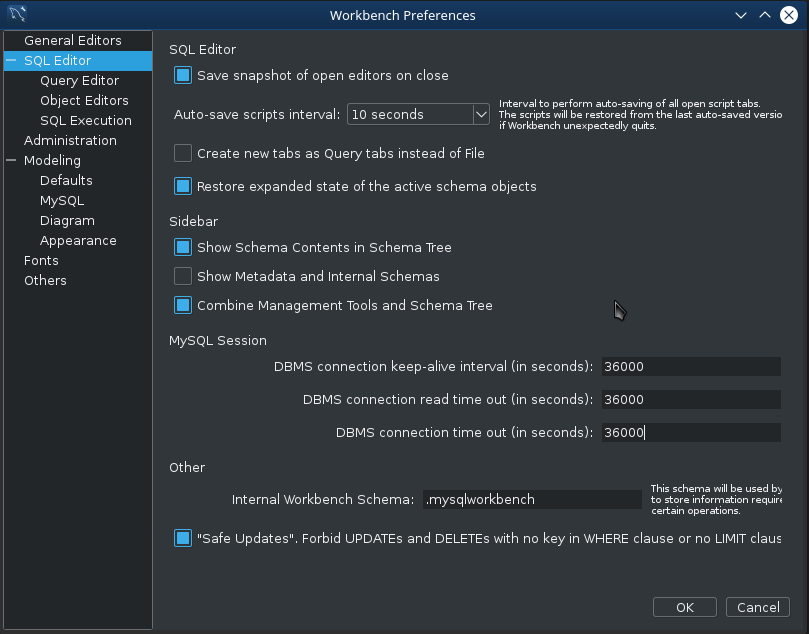
\includegraphics[width=0.6\textwidth]{mysql_wb_settings}
	\caption{MySQL Workbench: Setting timeout values to avoid connection loss}
	\label{fig:mysql_wb_settings}
\end{figure}
% space

\noindent
The next problem was the lack of disk space. 
MySQL by default stores all databases and belonging tables in /var/lib/mysql/, and it also creates temporary backup files 
(where the file size is equal to the size of the current database). 
Since the default folder for temporary files was on /root, the disk space was used up in less than 30 minutes. 
Therefore, two things needed to be done. First, disable the storage of temporary files, and secondly change the storage location for the database. 
The problem when tinkering with the configuration file is that things easily break. 
Which is what happened, and a clean install was needed for both MariaDB and MySQL (the changed settings can be seen in Listing  \ref{lst:mariadb_config_file}). 
The final step was to create symbolic links that linked the database to the  location where the tables were stored 
(this has to be done before creating the tables, if not MySQL  Workbench will store the tables in /var/lib/mysql/)\footnote{
	It should be noted that after an upgrade of MariaDB, MySQL and MariaDB could no longer find the tables, even if they still were in the /home/mysql/ folder. 
	It is therefore advisable to dump the database after inserting all the tables, since it goes a lot faster to restore the database from dump rather than insertion from XML files.
	}. 
% listing of changes made to config file (MariaDB)
\begin{lstlisting}[caption={Changes made to config file: /etc/mysql/my.cnf}, label={lst:mariadb_config_file}] 
# disable storage of temporary files
#tmpdir = /tmp/		  
# disable storage of log files
#log-bin = mysql-bin  

# set directory for storing database files
datadir = /home/mysql 
\end{lstlisting}

% Listing showing the SQL for loading XML row data into MySQL
\begin{lstlisting}[caption={Load XML file into a table in the MySQL database}, label={lst:load_xml_file}] 
LOAD XML LOCAL INFILE 
path_to_xml_file
INTO TABLE db_table
ROWS IDENTIFIED BY '<row>';
\end{lstlisting}

\noindent
Listing \ref{lst:load_xml_file} shows how the files were loaded into the tables, and the complete database can be seen in Appendix \ref{app:mysql_database}, p.~\pageref{app:mysql_database}. 
Since the Posts table is large (\textasciitilde 29,5 million rows) and it contains both questions and answers, two new tables were created; 
"posvote\_Posts"\footnote{
	The Posts table has a file size of \textasciitilde 43,6 GB, 
	whereas posvote\_Posts file size is \textasciitilde 11,2 GB. 
	negvote\_Posts has a file size of \textasciitilde 1,33 GB.
	} 
and "negvote\_Posts". 
posvote\_Posts contains questions with a score higher then zero (score > 0) and negvote\_Posts contains all questions with a score lower then zero (score < 0).

\section{Development process} 
\label{sec:libsvm_implementation}
When starting the development, the focus was on retrieving the data from the database, and processing it for text analysis. 
To be able to store all the retrieved columns and the belonging rows without creating object classes, the pandas.DataFrame\footnote{
	Pandas: \url{http://pandas.pydata.org/}.
	} 
was used. 
% add something a bit more detailed about pandas; what makes it good, etc.

The questions retrieved needed to be processed before any analysis could be done. 
The reason for this is because the questions was written as HTML (including HTML entities). 
An example is shown in Listing \ref{lst:unprocessed_question}. 
Every question starts with the <p> tag, and if the question contains code samples, these are wrapped with a <code> tag. 
To convert the HTML text into readable text, a HTML parser class was created (based on answer by \cite{Eloff2009}).
\newpage\noindent
% listing with question before HTML is removed
\begin{lstlisting}[caption={Question before HTML is removed (Question ID: 941156)}, 
label={lst:unprocessed_question}, basicstyle=\small] 
<p>
Why do we need callbacks in ASP.NET or any server side technology?
</p>&#xA;&#xA;<p>One answer can be, to achieve asynchronous calls. 
</p>&#xA;&#xA;<p>But I am not satisfied with this answer.</p>
&#xA;&#xA;<p>Please explain it in a different way.
</p>
&#xA;
\end{lstlisting}
% space

\noindent
To process the questions, CountVectorizer from scikit-learn was used. 
CountVectorizer uses the vocabulary found in the text and counts the frequency of each word \cite{Scikitlearn.org2016b} \cite[4.2.3]{Scikitlearn.org2016}. 
When looking at this vocabulary, a lot of of un-important words was found (a lot which came from the code samples) provided in some of the questions. 
At first all code samples were removed from the text, but later on they were replaced with the value 'has\_codeblock', indicating that this question contained one or more code samples. 
This was achieved by using a combination of lxml\footnote{lxml: \url{http://lxml.de/}} and bs4\footnote{BeatifulSoup: \url{https://www.crummy.com/software/BeautifulSoup/}} (BeatifulSoup). 
lxml was used to construct an XML tree containing all the tags (to be able to retrieve the content by searching for a given tag), and bs4 was used for beautifying the HTML 
(since in some cases an error was thrown complaining about "Missing end tag").
\vspace{0.5em}\newline
However, for some questions, part of the text was lost, and for others, some <code> tags was not removed. 
On inspection, it was found that the trailing text following the <code> samples was stored in a .tail attribute. 
Since the <code> was removed, the .tail attribute was also removed. 
This was fixed by storing the the content of the <code> .tail attribute into its <parent>\footnote{
	It was also necessary to check if the <parent> had a .tail, if not, the .tail attribute had to be set for the <parent> to avoid the error: 
	"NoneType + str: TypeError".
	} 
(where <parent> is the tag that contained the given <code></code>) .tail attribute. 
As for the non-complete removal of <code> tags, this error mostly occurred for code samples that contained XML or HTML code\footnote{
	One example is this question: \\
	\url{http://stackoverflow.com/questions/19535331/print-page-specific-area-or-element}.
	}, 
because the lxml parser failed. 
The solution was to replace the lxml parser with bs4 and just change the content of the <code> tag to the value 'has\_codeblock'.
\vspace{0.5em}\newline
Considering the size of the dataset, and that the source code was hosted on GitHub, I was hesitant to store the training data in a separate file. 
However, when loading 20,000 samples from the database with a 'WHERE' parameter, things tend to go more slow. 
At this point, it was decided to try to dump the loaded data from the database to a file. 
This was achieved by using pandas.DataFrame.to\_csv\footnote{
	pandas.DataFrame.to\_csv: \\
	\url{http://pandas.pydata.org/pandas-docs/stable/generated/pandas.DataFrame.to_csv.html}.
	}. 
At a later point, the unprocessed dataset was also dumped to a CSV file for replicability\footnote{The only change made to the unprocessed dataset was removing the HTML tags.}.
\vspace{0.5em}\newline
Further examination showed that the vocabulary contained a lot of numerical and hexadecimal values, but also a lot of non-English words. 
The numerical and hexadecimal values were replaced using regular expressions to 'has\_hexadecimal' and 'has\_numeric'. 
The non-English words were a bit more troublesome to handle, since these were mainly used to prove a point or show an example of the issue they were having\footnote{ 
	\url{http://stackoverflow.com/questions/856307/wordwrap-a-very-long-string}.
	}. 
Attempts were made to filter them out by using corpus.words.words() and corpus.wordnet.synset() 
from \gls{nltk}\footnote{\url{http://www.nltk.org/}}, and PyEnchant\footnote{\url{http://pythonhosted.org/pyenchant/}}. 
However, WordNet does not have a complete database of all English words, and they all claimed some words were not English even though they were.
\vspace{0.5em}\newline
The solution turned out to be a lot simpler. 
Instead of creating filters, the CountVectorizer already had one built in. 
By adjusting the minimum document frequency (min\_df) and set it to 0.01, it would ignore words that did not appear in less then 1\% of all documents.

~\\
To write: \\
Tutorials that I went through \\
Using SGD (based on tutorials from scikit-learn) \\
Testing out different text classification algorithms (SVC, SGD and LinearSVC) \\
Attempting to make program runnable from command line; e.g. started with opt/argparse, ended with while loop

\begin{comment}
	Timeline:
		1. Created retrieval method for bad questions from db
			1.1. Using pandas to store data retrieved from db
		2. Added HTML class to remove tags
			Answer source: \url{http://stackoverflow.com/a/925630}
			Source: \url{http://stackoverflow.com/questions/753052/strip-html-from-strings-in-python}
			Accepted answer: "answered May 29 '09 at 11:47 Eloff"
			And comment to this answer by 'pihentagyu aka James Doepp' (May 21 '15 at 17:49)
		3. Tutorial by: \url{http://radimrehurek.com/data_science_python/}
		4. Removal of codeblocks from the question
			4.1 Using BeatifulSoup to processes tags without end-tags			
			4.2 Issues with losing the tail (text after codeblock); attaching it to parent
			4.3 Issue "NoneType + str: TypeError". Caused by parent not having tail. 
				Fixed by adding a .tail and setting it to '' on the <parent>.
			4.4 HTML w/ XML causing issues; parser fails (because parser was also xml, adding xml 
				to beginning of text). Example: 
				\url{http://stackoverflow.com/questions/19535331/print-page-specific-area-or-element}
			4.5 Filtering out questions that failed by adding their index to a temp list, and then 
				removing them from dataset
		5. Issue: Scikit-learn documentation is for v17.1, whereas I was using developer version v18.0
		   (part of the issue was that it wasn't installable, so it was installed from GitHub repo instead)
		   considered switching to libsvm (which wasn't installable through pypi in the beginning)
		6. Instead of removing codeblocks, the text 'has\_codeblock' was added to indicate code was used
			6.1 Stored the processed questions to .csv
		7. Discovered data missing in some questions by looking at the CSV. 
		   Some <code> snippetes weren't removed. Content found after EOF
		   Issue 4.4 was fixed by removing all lxml conversion and using bs4 instead
		8. Questions start with <p>, this was removed by setting all text to be on one line
		9. Removal of numeric and hexadecimal values from text. Issue with trash data, e.g:
			\url{http://stackoverflow.com/questions/856307/wordwrap-a-very-long-string}
		10. Trash data: Using NLTK, NLTK.WordNet and enchant
			10.1 Tested out WordNet, could not discover english words. Does not contain all english words
			10.2 Tested out enchant, but could not in all cases either discover all english words
			10.3 Using Porter stemming to reduce features
			10.? \url{http://www.irfanelahi.com/data-science-document-classification-python/#Lexical-
			Analysis-of-the-Text-Data}
			10.? Setting min\_df=0.01 (ignore those occuring in less then 1\%) - helped a lot 
		11. Stemming of data, model creation and gridsearch with SGD			
		12. Model based on 20,000 samples (10k good, 10k bad) - took approx ~3hours for both models
			Model 1 was for all data (no test set). Model 2 was based on train\_test\_split
		13. Added tags column to the used dataset. Added the unprocessed dataset (but html is removed)
		14. Tested out different SVM algorithms (SVC, SGD and LinearSVC)
			Issue was that I managed to overwrite the .csv, so I had to do everything over again
			took approximately 24-36 hours to complete (+ 3days before hand to make everything run smoothly).
		15. Attempted to use optparse, argparse to make it executable. 
			Problem is that it exits after command is run. Need it to continue running to be able to:
				a) create new (or load existing) model
				b) use model from a) to predict quality of entered question (rinse/repeat)
		16. Used while loop instead (loop until exit entered). shortcuts are the same as with argparse, but 
			without the '-' in front (e.g. instead of -e, just press 'e' to exit)
			
		Additional Notes (which might be relevant for the next section):
		
			- issues with setting up environment, installations, etc
			- switching from "good"/"bad" to +/-1 for class label (bcz libsvm)
			- switching from -10/+50 to -5/+50 to get more separation (and more results for bad)
			
		Potentially useful links:
		
		http://billchambers.me/tutorials/2015/01/14/python-nlp-cheatsheet-nltk-scikit-learn.html
		http://stackoverflow.com/questions/28064634/random-state-pseudo-random-numberin-scikit-learn
		http://stackoverflow.com/questions/35382657/my-pipeline-configuration-for-text-classification-using-
		sklearn-in-python
\end{comment}

\section{Feature sets, attributes and processing}
\label{sec:feature_sets}
When retrieving the questions from the database, the vote score was set to less than -10 for bad question and greater than 50 for good questions (retrieval limit set to 10,000; 20,000 total). 
However, the vote score was set too low for the bad questions, since only 683 rows was returned. 
The score was then set to less than -5. 
When using pandas.Categorical to get an statistical overview (code snippet in Listing \ref{lst:pandas_categorical} and result in Table \ref{tab:pandas_categorical}), 
one can see that for 10,000 samples, the average vote score was -7. This could be an indicator that when a question has a vote score below -5, they are ignored.

\newpage
\begin{lstlisting}[caption={Getting Categorical data from pandas.DataFrame}, 
label={lst:pandas_categorical}, basicstyle=\small] 
from pandas import DataFrame, Categorical

# get statistics from pandas.DataFrame
temp_df = __so_dataframe.loc[:, ("Score", "Body", "Title", 
	"AnswerCount", "length")]
temp_df.loc[:, CLASS_LABEL_KEY] = Categorical(__so_dataframe.loc[:, 
							"label"])

# prints out the questions AnswerCount, Score and length
print(temp_df.groupby("label").describe())
# prints all selected columns
print(temp_df.groupby("label").describe(include='all'))
\end{lstlisting}

\begin{table}[tbp]
	\centering
	\begin{tabular}{| c | c | c | c |c |}
		\hline
		Class 		& Statistics	& AnswerCount		& Score 		& Question length 	\\ \hline
		~ 			& ~ 			& ~  				& ~ 			& ~					\\ \hline
		% Bad Questions
		-1 			& mean 		& 2.0483 			& -7.0275 		& 319.226 		\\ \hline
		~ 			& std 		& 1.3129 			& 2.676 		& 382.115  		\\ \hline
		~ 			& min 		& 0.0 				& -147.0 		& 13.0  		\\ \hline
		~ 			& 25\% 		& 1.0 				& -7.0 			& 153.0 		\\ \hline
		~ 			& 50\% 		& 2.0 				& -6.0 			& 239.0  		\\ \hline
		~ 			& 75\% 		& 3.0 				& -6.0 			& 379.0  		\\ \hline
		~ 			& max 		& 20.0 				& -6.0 			& 13673.0  		\\ \hline
		% space
		~ 			& ~ 		& ~  				& ~ 			& ~				\\ \hline
		% Good Questions
		1 			& mean 		& 11.9379 			& 182.5483 		& 459.329		\\ \hline
		~ 			& std 		& 13.707824			& 317.47217 	& 531.187559  		\\ \hline
		~ 			& min 		& 0.0 				& 51.0 			& 13.0  		\\ \hline
		~ 			& 25\% 		& 6.0 				& 67.0 			& 189.0 		\\ \hline
		~ 			& 50\% 		& 9.0 				& 96.0 			& 328.0  		\\ \hline
		~ 			& 75\% 		& 14.0 				& 173.0 		& 558.0  		\\ \hline
		~ 			& max 		& 518.0 			& 9432.0 		& 18867.0  		\\ \hline
		
	\end{tabular}
	\caption{Results from pandas.DataFrame and pandas.Categorical. -1 is for bad questions (votes < -5), 
		and 1 are for good questions (votes > 50).}
	\label{tab:pandas_categorical}
\end{table}

\begin{table}[tbp]
	\centering
	\begin{tabular}{| c | c | c | c |}
		\hline
		Step & Text processing  & Vocabulary count & CountVectorizer  \\ \hline
		1 	& None 									& 69766 	& analyzer="word" \\ \hline
		2 	& Stop words 							& 69462 	& 
			\shortstack{analyzer="word", \\ stop\_words="english"} \\ \hline
		3 	& \shortstack{Removal of code, 
			hexadecimal \\ and numerical values} 	& 27624 	& 
			\shortstack{analyzer="word", \\ stop\_words="english"} \\ \hline
		4 	& Minimum document frequency 			& 440 		& 
				\shortstack{analyzer="word", min\_df=0.01, \\ stop\_words="english"} \\ \hline
	\end{tabular}
	\caption{Feature reduction steps before and after text was processed.}
	\label{tab:feature_reduction}
\end{table}

what features were selected and why? \\
how was data processed (e.g. retrieved from db, converted to scikit-learn format, and so forth) \\
attributes: length, symbols, question sentence only, code snippet, votes, closed, etc.

\newpage
Hypotheses drafts (need to be re-written)
\begin{itemize}
	\item Does the use of stemming increase the \gls{svm}s accuracy?
	\item Does the use of tags increase the \gls{svm}s accuracy?
	\item If a question has version numbering, does this increase \gls{svm}s accuracy?
	\item Does syntax errors have an impact on the question (may not be tested due to LINT check)?
	\item If question contains links to sources (e.g. repository, StackOverflow question, etc), does it have any effect?
	\item What about questions containing homework description (e.g. homework, assignment, textbook, etc)?
\end{itemize}
